\chapter{Analysis of Production terms in Dynamos with Sustained Wreaths}
\label{chapter:dynamo production}
\label{sec:dynamo_production}
The magnetic wreaths formed in case~D3 are dominated by strong 
mean longitudinal field components and show little variation in time. 
To understand the physical processes responsible
for maintaining these magnetic wreaths, we examine the terms arising in
the time- and azimuth-averaged induction equation for case~D3.  
We derive diagnostic tools to evaluate the generation and transport of 
magnetic field in a magnetized and rotating turbulent convection
zone.  This derivation is in spherical coordinates, and is under the
anelastic approximation.

\section{Production of Axisymmetric Toroidal Field}
We begin our analysis by exploring the maintenance of the mean
toroidal field $\langle B_\phi \rangle$.  Here it is helpful to break
the induction term from equation~(\ref{eq:induction}) into
contributions from shear, advection and compression.
In the induction equation (\ref{eq:induction}), the first term on
the right hand side represents production of magnetic field while the
second term represents its diffusion.  We rewrite the production
term to make the contributions of shear, advection and compressible
effects more explicit as
\begin{equation}
  \nab\cross(\VV\cross\BB) = (\BB\cdot\nab)\VV-(\VV\cdot\nab)\BB-\BB(\Div\VV).
\end{equation}
Under the anelastic approximation the divergence of $\vec{v}$ can be
expressed in terms of the logarithmic derivative of the mean density because
\begin{equation}
  \Div(\rb \VV)=0=\rb(\Div \VV)+(\VV\cdot\nab)\rb, \nonumber
\end{equation}
and therefore
\begin{equation}
  \Div\VV=-v_r\frac{\p}{\p r}\ln \rb.
\end{equation}
The induction equation thus becomes
\begin{equation}\label{eq:ind2}
\frac{\p \BB}{\p t}=\underbrace{(\BB\cdot\nab)\VV}_{\mbox{shearing}}
                   -\underbrace{(\VV\cdot\nab)\BB}_{\mbox{advection}}
		   +\underbrace{v_r\BB\frac{\p}{\p r}\ln \rb}_{\mbox{compression}}
		   -\underbrace{\nab\cross(\eta\nab\cross\BB)}_{\mbox{diffusion}}
\end{equation}
As labeled, the first term represents shearing of $\BB$, the second
term advection of $\BB$, the third one compressible amplification
of $\BB$, and the last term ohmic diffusion.

To identify the processes contributing to the production of mean
(axisymmetric) field, we separate our velocities and magnetic fields
into mean and fluctuating components 
$\vec{v} = \langle \vec{v} \rangle  + \vec{v}' $ and
$\vec{B} = \langle \vec{B} \rangle  + \vec{B}' $ 
where angle brackets denote an average in longitude.  Thus 
$\langle \vec{v}' \rangle = \langle \vec{B}' \rangle = 0$ by definition.
Expanding the production term of equation~(\ref{eq:ind2}) we obtain the
mean shearing term
\begin{equation}
  \langle (\BB\cdot\nab)\VV \rangle = \left( \langle \BB \rangle \cdot\nab \right) \langle \VV \rangle 
                                    + \langle (\vec{B}'\cdot\nab)\vec{v}' \rangle,
\end{equation}
the mean advection term
\begin{equation}
  -\langle (\VV\cdot\nab)\BB \rangle = -\left( \langle \VV \rangle \cdot\nab \right) \langle \BB \rangle 
                                       -\langle (\vec{v}'\cdot\nab)\vec{B}' \rangle,
\end{equation}
and the mean compressibility term
\begin{equation}
  \langle v_r\BB\frac{\p}{\p r}\ln \rb \rangle = \left( \langle v_r \rangle \langle \BB \rangle  
                                              +  \langle v_r' \vec{B}' \rangle \right)\frac{\p}{\p r}\ln \rb.
\end{equation}
In a similar fashion, the mean diffusion term becomes
\begin{equation}
  -\langle \nab\cross(\eta\nab\cross\BB) \rangle = -\nab\cross(\eta\nab\cross \langle \BB \rangle).
\end{equation}

The axisymmetric component of the induction equation is written
symbolically as:

\begin{equation}
  \label{eq:mean induction}
  \frac{\partial \langle \vec{B} \rangle }{\partial t} = P_\mathrm{MS} + P_\mathrm{FS} 
                                      + P_\mathrm{MA} + P_\mathrm{FA} 
				      + P_\mathrm{MC} + P_\mathrm{FC}
                                      + P_\mathrm{MD}
\end{equation}
With $P_\mathrm{MS}$ representing production of field by mean shear,
     $P_\mathrm{FS}$ production by fluctuating shear,
     $P_\mathrm{MA}$ advection by mean flows, 
     $P_\mathrm{FA}$ advection by fluctuating flows, 
     $P_\mathrm{MC}$ amplification arising from the compressibility of
     mean flows, $P_\mathrm{FC}$ amplification arising from
     fluctuating compressible motions, and 
     $P_\mathrm{MD}$ ohmic diffusion of the mean fields.  In turn,
     these terms are
%\begin{eqnarray}
\begin{align}\label{eq:mean terms}
  P_\mathrm{MS} =& \left( \langle \BB \rangle \cdot\nab \right)\langle \VV \rangle\thinspace, & % \qquad \qquad %\\
  P_\mathrm{FS} =& \langle (\vec{B}'\cdot\nab)\vec{v}' \rangle\thinspace, \notag \\
  P_\mathrm{MA} =& -\left( \langle \VV \rangle \cdot\nab \right) \langle \BB \rangle\thinspace,& %  \qquad \qquad %\\
  P_\mathrm{FA} =& -\langle (\vec{v}'\cdot\nab)\vec{B}'  \rangle\thinspace,   \\   \label{eq:mean terms}
  P_\mathrm{MC} =&  \left( \langle v_r \rangle \langle \BB \rangle \right)\frac{\p}{\p r}\ln \rb\thinspace, & % \qquad \qquad %\\
  P_\mathrm{FC} =&  \left( \langle v_r' \vec{B}' \rangle \right)\frac{\p}{\p r}\ln \rb\thinspace, \notag\\
  P_\mathrm{MD} =& -\nab\cross(\eta\nab\cross \langle \BB \rangle)\thinspace. & &\notag
\end{align}
%\end{eqnarray}
We now expand each of these terms into their full representation in spherical coordinates.

\begin{eqnarray}\label{eq:ind3pe}
 \frac{\partial \langle B_{\phi} \rangle }{\partial t} &=&
             P_\mathrm{MS} + P_\mathrm{FS}  
	   + P_\mathrm{MA} + P_\mathrm{FA} 
	   + P_\mathrm{MC} + P_\mathrm{FC}
	   + P_\mathrm{MD} \nonumber\\
%
\label{eq:MS phi}
P_\mathrm{MS} &=& \phn\advbm  \langle v_{\phi} \rangle  + \frac{ \langle B_{\phi} \rangle  \langle v_r \rangle  + \cot\theta  \langle B_{\phi} \rangle  \langle v_{\theta} \rangle }{r}\\
\label{eq:FS phi}
P_\mathrm{FS} &=& \phn\bigg\langle \advbf v_{\phi}' \bigg\rangle  + \frac{ \langle B_{\phi}'v_r' \rangle  + \cot\theta  \langle B_{\phi}'v_{\theta}' \rangle }{r}\\
\label{eq:MA phi}
P_\mathrm{MA} &=& -\advvm  \langle B_{\phi} \rangle  - \frac{ \langle v_{\phi} \rangle  \langle B_r \rangle  + \cot\theta  \langle v_{\phi} \rangle  \langle B_{\theta} \rangle }{r}  \\
\label{eq:FA phi}
P_\mathrm{FA} &=& -\bigg\langle \advvf B_{\phi}' \bigg\rangle  - \frac{ \langle v_{\phi}'B_r' \rangle  + \cot\theta  \langle v_{\phi}'B_{\theta}' \rangle }{r} \\
\label{eq:MC phi}
P_\mathrm{MC} &=& \phn\left(\langle v_r \rangle  \langle B_{\phi} \rangle\right)\frac{\p}{\p r}\ln \rb \thinspace, \qquad\qquad \qquad%\\
\label{eq:FC phi}
P_\mathrm{FC} = \left(\langle v_r'B_{\phi}' \rangle \right)\frac{\p}{\p r}\ln \rb\\
\label{eq:MD phi}
P_\mathrm{MD} &=& \phn\eta\nabla^{2} \langle B_{\phi} \rangle -\frac{\eta  \langle B_{\phi} \rangle }{r^2\sin^2\theta}+\frac{d\eta}{dr}\left(\frac{1}{r}\frac{\p (r \langle B_{\phi} \rangle )}{\p r} \right) 
\end{eqnarray}



\section{Maintaining Wreaths of Toroidal Field}
The evolution of the mean longitudinal (toroidal) field $\langle B_\phi \rangle$
is described symbolically in equation~(\ref{eq:mean induction}), with
individual terms defined in equation~(\ref{eq:mean terms}).
When we analyze these terms in case~D3, we find that  $\langle
B_\phi \rangle$ is produced by the shear of differential rotation and
is dissipated by a combination of turbulent induction and ohmic
diffusion.  This balance can be restated as  
\begin{equation}
  \frac{\partial \langle B_\phi \rangle}{\partial t} \approx 
  P_\mathrm{MS} + \left(P_\mathrm{FS} + P_\mathrm{FA} + P_\mathrm{MD}\right)
  \approx 0\thinspace ,
\end{equation}
with $P_\mathrm{MS}$ representing production by the mean shearing flow of
differential rotation, 
$P_\mathrm{FS}$ by fluctuating shear, $P_\mathrm{FA}$ by fluctuating
advection, and $P_\mathrm{MD}$ by mean ohmic diffusion.
Those terms are in turn 
\begin{eqnarray}
  \label{eq:P_DR}
  P_\mathrm{MS} &=& \phn\left(\langle \vec{B} \rangle \cdot \vec{\del} \right) 
    \langle \vec{v} \rangle \big|_\phi, \\
  \label{eq:P_turb}
  P_\mathrm{FS} &=& \phn\left\langle \left(\vec{B}' \cdot \vec{\del} \right)  
    \vec{v'} \right\rangle\big|_\phi, \\
  P_\mathrm{FA} &=& - \left\langle \left(\vec{v}' \cdot \vec{\del} \right) 
    \vec{B'} \right\rangle\big|_\phi, \\
  \label{eq:P_diff}
  P_\mathrm{MD} &=& -\vec{\del} \cross \eta \vec{\del} \cross \langle
    \vec{B} \rangle \big|_\phi,
\end{eqnarray}
where brackets again indicate an azimuthal average and primes
indicate fluctuating terms: $\vec{v}' = \vec{v} - \langle \vec{v} \rangle$.
The detailed implementation of these terms  is presented for our
spherical geometry in equations~(\ref{eq:MS phi}-\ref{eq:MD phi}).
These terms are illustrated in Figure~\ref{fig:D3_bphi_production}
for case~D3, averaged over a 450~day interval from day~6450~to~6900.  

The structure of $\langle B_\phi \rangle$ is shown in
Figure~\ref{fig:D3_bphi_production}$a$.  The shearing flows of
differential rotation $P_\mathrm{MS}$
(Fig.~\ref{fig:D3_bphi_production}$b$) act almost everywhere to
reinforce the mean toroidal field.  Thus the polarity of this production term
generally matches that of $\langle B_\phi \rangle$.  This production is balanced by
destruction of mean field arising from both turbulent induction and ohmic diffusion
(sum shown in Fig.~\ref{fig:D3_bphi_production}$c$).  The individual
profiles of $P_\mathrm{FS}$, $P_\mathrm{FA}$ and $P_\mathrm{MD}$ are
presented in turn in Figures~\ref{fig:D3_bphi_production}$d,e,f$.
The terms from turbulent induction ($P_\mathrm{FS}$ and
$P_\mathrm{FA}$) contribute to roughly half of the total balance, with
the remainder carried by ohmic diffusion of the mean fields
($P_\mathrm{MD}$).  In the core of the wreaths, removal of mean
toroidal field is largely accomplished
by fluctuating advection $P_\mathrm{FA}$
(Fig.~\ref{fig:D3_bphi_production}$e$) and mean ohmic diffusion
$P_\mathrm{MD}$ (Fig.~\ref{fig:D3_bphi_production}$f$), with the latter also important near the upper boundary.
Turbulent shear becomes strongest
near the bottom of the convection zone and in the
regions near the high-latitude side of each wreath.
Thus $P_\mathrm{FS}$ (Fig.~\ref{fig:D3_bphi_production}$d$) becomes the dominant member of the triad of terms
seeking to diminish the mean toroidal field there. 
We find that the mean poloidal field is regenerated in roughly the
same region.

%\begin{sidewaysfigure}
\begin{figure}[!t]
%  \vskip-2cm
  \begin{center}
    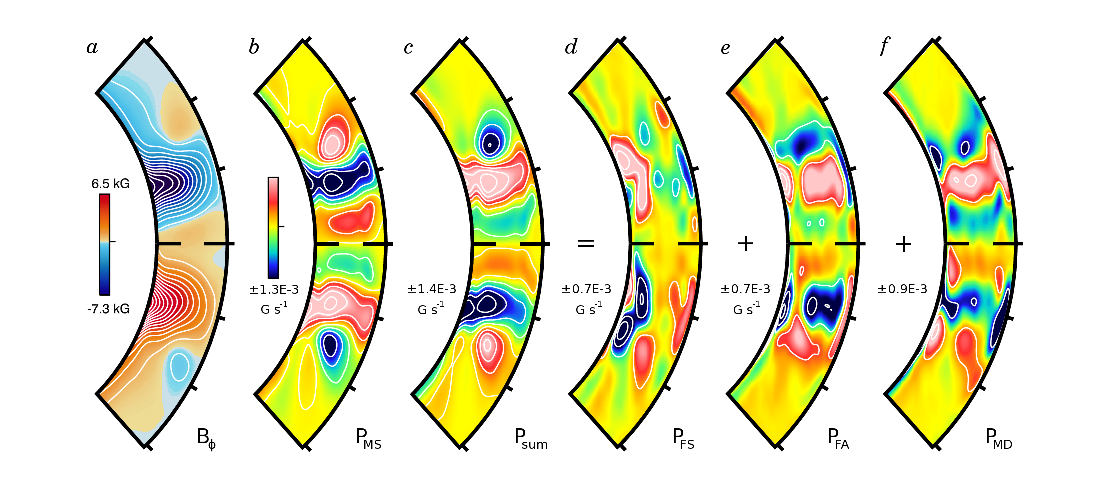
\includegraphics[width=\linewidth]{figs/chapter_7/Figure_13/Figure_13.eps}
  \end{center}
  \caption[Generation of $\langle B_\phi \rangle$ in case~D3]
          {Generation of $\langle B_\phi \rangle$ in case~D3.  
    The view is from $\pm 45^\circ$ latitude to emphasize the
    equatorial regions.  $(a)$~Mean toroidal field $\langle B_\phi
    \rangle$ with wreaths strongly evident.  $(b)$~Production by
    $P_\mathrm{MS}$ serves to build $\langle B_\phi \rangle$.
    This rate term generally matches the sense of $\langle B_\phi \rangle$,
    thus being negative (blue in colorbar, with ranges indicated) in the core of the
    northern wreath and positive (red) in that of the southern wreath.
    $(c)$~Destruction of mean toroidal field is achieved by the sum of
    the two fluctuating (turbulent) induction terms and the ohmic
    diffusion $\left(P_\mathrm{FS} + P_\mathrm{FA} + P_\mathrm{MD}\right)$.
    This sum clearly has opposite sense and similar magnitude to $P_\mathrm{MS}$.  
    We break out these three destruction terms in the following panels.
    $(d)$~Fluctuating (turbulent) shear
    $P_\mathrm{FS}$ is strongest near the high-latitude side of each
    wreath, and $(e)$~fluctuating (turbulent) advection $P_\mathrm{FA}$ is strongest
    in the cores of the wreaths.  The sum of these terms
    $\left(P_\mathrm{FS} + P_\mathrm{FA}\right)$ is
    responsible for about half the destructive balance, with the
    remainder coming from $(f)$~the mean ohmic diffusion $P_\mathrm{MD}$.
    Some differences arise in the boundary layers at top and bottom.
    \label{fig:D3_bphi_production}}
\end{figure}
%\end{sidewaysfigure}

In the analysis presented in Figure~\ref{fig:D3_bphi_production} we have
neglected the advection of $\langle B_\phi \rangle$ 
by the meridional circulations (denoted by $P_\mathrm{MA}$), which we find plays a very small role
in the overall balance.  We have also neglected the amplification of
$\langle B_\phi \rangle$ by compressibility effects (namely, 
$P_\mathrm{MC}$ and $P_\mathrm{FC}$), though it does
contribute slightly to reinforcing the underlying mean fields within
the wreaths.

To summarize, the mean toroidal fields are built through an
$\Omega$-effect, where production by the mean shearing flow of
differential rotation ($P_\mathrm{MS}$) builds the underlying
$\langle B_\phi \rangle$.  In the statistically steady state achieved, this
production is balanced by a combination of turbulent
induction ($P_\mathrm{FS} + P_\mathrm{FA}$) and ohmic diffusion of the
mean fields ($P_\mathrm{MD}$).

\section{Production of Axisymmetric Poloidal Field}
%Still not entirely happy about this lead in \textbf{7/24/09} 

When analyzing the production of the mean poloidal field, two
contributions arise.  One is for the mean radial field and one for the
mean colatitudinal field.  Evaluating the production of poloidal field
in terms of the radial and colatitudinal field is a bit complex, and
in practice the production of the mean poloidal vector potential is a
more useful quantity.  For clarity however, it is useful to first exhibit
the production terms for radial and colatitudinal in a fashion similar to 
those evaluated for the mean toroidal field.  With the same analysis approach,
the induction equation for those two fields are in turn
\begin{eqnarray}
\frac{\partial \langle B_{r} \rangle }{\partial t} &=&
             P_\mathrm{MS} + P_\mathrm{FS}  
	   + P_\mathrm{MA} + P_\mathrm{FA} 
	   + P_\mathrm{MC} + P_\mathrm{FC}
	   + P_\mathrm{MD} \nonumber\thinspace,\\
P_\mathrm{MS} &=& \phn\advbm  \langle v_r \rangle  - \frac{ \langle B_{\theta} \rangle  \langle v_{\theta} \rangle + \langle B_{\phi} \rangle  \langle v_{\phi} \rangle }{r}\thinspace,\\
P_\mathrm{FS} &=& \phn\bigg\langle \advbf v_r' \bigg\rangle  - \frac{ \langle B_{\theta}'v_{\theta}' \rangle + \langle B_{\phi}'v_{\phi}' \rangle }{r}\thinspace,\\
P_\mathrm{MA} &=&-\advvm  \langle B_r \rangle  + \frac{ \langle v_{\theta} \rangle  \langle B_{\theta} \rangle + \langle v_{\phi} \rangle  \langle B_{\phi} \rangle }{r}\thinspace,\\
P_\mathrm{FA} &=&-\bigg\langle \advvf B_r' \bigg\rangle  + \frac{ \langle v_{\theta}'B_{\theta}' \rangle + \langle v_{\phi}'B_{\phi}' \rangle }{r}\thinspace,\\
P_\mathrm{MC} &=& \phn\left( \langle v_r \rangle  \langle B_r \rangle
             \right)\frac{\p}{\p r}\ln \rb\thinspace, \qquad\qquad \qquad %\\
P_\mathrm{FC} = \left( \langle v_r'B_r' \rangle \right)\frac{\p}{\p r}\ln \rb\thinspace,\\
P_\mathrm{MD} &=& \phn\eta\nabla^{2} \langle B_r \rangle 
                - 2\eta\frac{ \langle B_r \rangle }{r^2}
		- \frac{2\eta}{r^2}\frac{\p \langle B_{\theta} \rangle }{\p \theta}
                - \frac{2\eta \cot\theta \langle B_{\theta} \rangle }{r^2}\thinspace,
\end{eqnarray}
and
\begin{eqnarray}
\frac{\partial \langle B_{\theta} \rangle }{\partial t} &=&
             P_\mathrm{MS} + P_\mathrm{FS}  
	   + P_\mathrm{MA} + P_\mathrm{FA} 
	   + P_\mathrm{MC} + P_\mathrm{FC}
	   + P_\mathrm{MD}\thinspace, \nonumber\\
P_\mathrm{MS} &=& \phn\advbm  \langle v_{\theta} \rangle  + \frac{ \langle B_{\theta} \rangle  \langle v_r \rangle - \cot\theta  \langle B_{\phi} \rangle  \langle v_{\phi} \rangle }{r}\thinspace,\\
P_\mathrm{FS} &=& \phn\bigg\langle \advbf v_{\theta}' \bigg\rangle  + \frac{ \langle B_{\theta}'v_r' \rangle -\cot\theta  \langle B_{\phi}'v_{\phi}' \rangle }{r}\thinspace,\\
P_\mathrm{MA} &=& -\advvm  \langle B_{\theta} \rangle  - \frac{ \langle v_{\theta} \rangle  \langle B_r \rangle -\cot\theta  \langle v_{\phi} \rangle  \langle B_{\phi} \rangle }{r}\thinspace,\\
P_\mathrm{FA} &=& -\bigg\langle \advvf B_{\theta}' \bigg\rangle  - \frac{ \langle v_{\theta}'B_r' \rangle - \cot\theta  \langle v_{\phi}'B_{\phi}' \rangle }{r}\thinspace,\\
P_\mathrm{MC} &=& \phn\left( \langle v_r \rangle  \langle B_{\theta} \rangle \right)\frac{\p}{\p r}\ln \rb\thinspace,  \qquad\qquad \qquad%\\
P_\mathrm{FC} = \phn\left(\langle v_r'B_{\theta}' \rangle \right)\frac{\p}{\p r}\ln \rb\thinspace,\\[3mm]
P_\mathrm{MD} &=&\phn\eta\nabla^{2} \langle B_{\theta} \rangle 
                 +\frac{2\eta}{r^2}\frac{\p \langle B_r \rangle }{\p \theta}
                 -\frac{\eta  \langle B_{\theta} \rangle}{r^2\sin^2\theta} \nonumber\\[3mm]
	& &\qquad\qquad\qquad + \frac{d\eta}{dr}\left(\frac{1}{r}\frac{\p (r \langle B_{\theta} \rangle )}{\p r}-\frac{1}{r}\frac{\p  \langle B_r \rangle }{\p \theta} \right).
\end{eqnarray}
In practice we use the above equations to diagnose and understand the
local production of poloidal field, but will not show these terms
explicitly.  

Instead, we find that when analyzing the production of mean poloidal
magnetic field, the balances achieved are somewhat clearer if we
consider its vector potential rather than the two separate
fields themselves.  The mean poloidal field 
$\langle \vec{B}_\mathrm{pol} \rangle$ has a corresponding vector
potential $\langle A_\phi \rangle$, where  
\begin{equation}
  \label{eq:poloidal decomposition}
  \begin{array}{rl}
    \displaystyle
    \langle \vec{B}_\mathrm{pol} \rangle &= \langle B_r \rangle \vec{\hat{r}} +
    \langle B_\theta \rangle \vec{\hat{\theta}} = \vec{\del} \cross \langle \vec{A}\big|_\phi \rangle \\[3mm]
    \displaystyle
    &= \frac{1}{r \sin \theta} \frac{\partial}{\partial \theta}
    \left\langle A_\phi \sin \theta \right\rangle \vec{\hat{r}} - 
    \frac{1}{r} \frac{\partial}{\partial r} \left\langle r A_\phi \right\rangle \vec{\hat{\theta}} \\[3mm]
    \displaystyle
    &= \vec{\del} \cross \left\langle A_\phi \vec{\hat{\phi}} \right\rangle.
  \end{array}
\end{equation}

The other components of the poloidal vector potential disappear, as terms involving
$\partial/\partial \phi$ vanish in the azimuthally-averaged equations.  
Likewise, the $\phi$-component of the possible gauge term $\vec{\del} \lambda$ is zero by
virtue of axisymmetry.
We recast the induction equation (eq.~\ref{eq:induction}) in terms of
the poloidal vector potential by uncurling the equation once and obtain
\begin{equation}
  \label{eq:A induction}
    \frac{\partial\langle\vec{A_\phi}\rangle}{\partial t} = 
        \vec{v} \cross \vec{B}{\big|}_\phi - \eta \vec{\del} \cross
        \vec{B}{\big|}_\phi.
\end{equation}
This can then be decomposed into mean and fluctuating contributions,
and represented symbolically as 
\begin{equation}
  \label{eq:A induction symbolic}
    \frac{\partial\langle\vec{A_\phi}\rangle}{\partial t} = 
        E_\mathrm{MI} + E_\mathrm{FI} + E_\mathrm{MD},
\end{equation}
with $E_\mathrm{MI}$ representing the electromotive forces (emf)
arising from mean flows and mean fields, and related to their mean
induction.  Likewise, $E_\mathrm{FI}$ is
the emf from fluctuating flows and fields and $E_\mathrm{MD}$ is 
the emf arising from mean diffusion.  These are in turn
\begin{eqnarray}
  \label{eq:A MI phi}
  E_\mathrm{MI} &= \phn\langle \vec{v} \rangle \cross \langle \vec{B} \rangle{\big|}_\phi
                 =& \langle v_r \rangle \langle B_\theta \rangle - 
                    \langle v_\theta \rangle \langle B_r \rangle, \\
  \label{eq:A FI phi}
  E_\mathrm{FI} &= \phn\langle \vec{v'}\cross\vec{B'} \rangle{\big|}_\phi
                 =& \langle v_r' B_\theta' \rangle - 
                    \langle v_\theta' B_r' \rangle, \\
  \label{eq:A MD phi}
  E_\mathrm{MD} &= -\eta \vec{\del} \cross \langle \vec{B} \rangle{\big|}_\phi 
                 =& -\eta \frac{1}{r} \left(\frac{\partial}{\partial r} 
		    \left(r \langle B_\theta \rangle \right)
		    - \frac{\partial \langle B_r \rangle}{\partial \theta}\right)\thinspace. 
\end{eqnarray}



\section{Maintaining the Poloidal Field}
The production of mean poloidal field is achieved through a slightly
different balance, with turbulent induction producing poloidal field and
ohmic diffusion acting to dissipate it.  The mean flows play
only a modest role in the overall balance.  

In case~D3 we find that the mean poloidal vector potential 
$\langle A_\phi \rangle$ is produced by the fluctuating (turbulent) emf and is
dissipated by ohmic diffusion
\begin{equation}
  \label{eq:poloidal balance}
  \frac{\partial \langle A_\phi \rangle}{\partial t} \approx 
  E_\mathrm{FI} +
  E_\mathrm{MD} \approx 0\thinspace,
\end{equation}
with $E_\mathrm{FI}$ the emf arising from fluctuating flows and
fluctuating fields, and contributing to the mean induction.  The
$E_\mathrm{MD}$ is the emf arising from mean
ohmic diffusion.  These terms are
\begin{eqnarray}
  \label{eq:E_FI}
  E_\mathrm{FI} &=& \langle \vec{v'}\cross\vec{B'} \rangle{\big|}_\phi
  = \langle v_r' B_\theta' \rangle - 
    \langle v_\theta' B_r' \rangle, \\
  E_\mathrm{MD} &=& -\eta \vec{\del} \cross \langle \vec{B} \rangle{\big|}_\phi.
\end{eqnarray}
The contribution arising from the omitted term $E_\mathrm{MI}$ 
(see~eq.~\ref{eq:A MI phi}), related to the emf of mean flows and mean
fields, is smaller than these first two by more than an order
of magnitude.  Additionally, $E_\mathrm{MI}$ has a complicated spatial
structure which does not appear to act in a coherent fashion within
the wreaths to either build or destroy mean poloidal field.

\begin{figure}[!tp]
  \begin{center}
    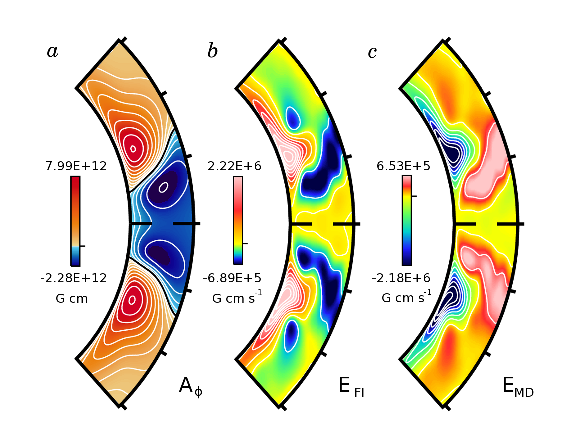
\includegraphics[width=0.7\linewidth]{figs/chapter_7/Figure_14/Figure_14.eps}
  \end{center}
  \caption[Production of mean poloidal vector potential $\langle A_\phi \rangle$ in case~D3]
          {Production of mean poloidal vector potential $\langle A_\phi \rangle$ in case~D3.  
    The view is restricted to $\pm 45^\circ$ latitude to emphasize the
    regions of production.  $(a)$~Mean poloidal vector potential  
    $\langle A_\phi \rangle$, with sense denoted by color (red,
    clockwise; blue, counter-clockwise).
    $(b)$~The fluctuating (turbulent) emf
    $E_\mathrm{FI}$ acts to build the vector potential.  
    This term is strongest near the bottom of the convection zone and
    the poleward side of the wreaths.  
    $(c)$~Mean ohmic diffusion $E_\mathrm{MD}$ acts everywhere in
    opposition to $E_\mathrm{FI}$.  
    The cores of the wreaths are positioned at roughly
    $\pm15^\circ$ latitude (Fig.~\ref{fig:D3_bphi_production}$a$).
  \label{fig:D3 poloidal production}}
%  \vskip0.1truein
\end{figure}

The mean vector potential $\langle A_\phi \rangle$ is shown in Figure~\ref{fig:D3 poloidal
production}$a$, with poloidal field lines represented by the overlying contours.  
The mean radial magnetic field $\langle B_r \rangle$ is
about $\pm 1$~kG in the cores of the wreaths, whereas the mean colatitudinal
field $\langle B_\theta \rangle$ has an amplitude of roughly $-2$~kG
(thus directed northward in both hemispheres),
concentrated near the bottom of the convection zone.

\clearpage
The production of $\langle A_\phi \rangle$ by the fluctuating (turbulent) emf
$E_\mathrm{FI}$ is shown in Figure~\ref{fig:D3 poloidal production}$b$.  
Here too we average over the same 450~day interval.
This term generally acts to reinforce the
existing poloidal field, having the same sense as the underlying
vector potential in most regions.  It is strongest near the bottom of
the convection zone and is concentrated at the poleward  side of
each wreath.  This is similar, though not identical, to the structure
of destruction of mean toroidal field by fluctuating shear $P_\mathrm{FS}$
(Fig.~\ref{fig:D3_bphi_production}$d$).  It suggests that mean 
toroidal field is here being converted into mean poloidal field by the
fluctuating flows.  

There are two terms that contribute to $E_\mathrm{FI}$, as shown in equation~(\ref{eq:E_FI}).
Much of that fluctuating emf arises from
correlations between fluctuating latitudinal flows and radial fields
$\langle -v_\theta'B_r' \rangle$, which follows the structure of $E_\mathrm{FI}$
(Fig.~\ref{fig:D3 poloidal production}$b$) closely.  The contribution from
fluctuating radial flows and colatitudinal fields $\langle
v_r'B_\theta'\rangle$ is more complex in structure.  
Near $\pm 20^\circ$ latitude, this term reinforces
$\langle -v_\theta'B_r' \rangle$, but acts against it at
higher latitudes and thus diminishes the overall amplitude of
$E_\mathrm{FI}$. 
The mean ohmic diffusion $E_\mathrm{MD}$ (Fig.~\ref{fig:D3
  poloidal production}$c$), almost entirely balances the production of
$\langle A_\phi \rangle$ by $E_\mathrm{FI}$.

This shows that our mean poloidal magnetic field is maintained by the
fluctuating (turbulent) emf and is destroyed by ohmic diffusion.  In
mean-field dynamo theory, this is often parametrized by an
``$\alpha$-effect.''  Now we turn to interpretations within that framework.

\section{Exploring Mean-Field Interpretations}

Many mean-field theories assert that the production of mean poloidal
field is likely to arise from the fluctuating emf.  This process is often
approximated with an $\alpha$-effect, where it is proposed that the
sense and amplitude of the emf scales with the mean toroidal field
\begin{equation}
  \label{eq:mean field emf}
    \langle \vec{v'}\cross\vec{B'} \rangle = \alpha \langle \vec{B} \rangle,
\end{equation}
where $\alpha$ can be either a simple scalar or may be related to the
kinetic and magnetic (current) helicities.  In isotropic (but not
reflectionally symmetric), homogeneous, incompressible MHD turbulence 
\begin{eqnarray}
    \label{eq:mean-field alpha}
    \alpha  &=&\phn\frac{\tau}{3} \left(\alpha_k + \alpha_m \right), \\
    \label{eq:mean-field alpha_k}
    \alpha_k &=& -\vec{v'} \cdot \left(\vec{\del} \cross \vec{v'} \right), \\
    \label{eq:mean-field alpha_m}
    \alpha_m &=& \phn\frac{1}{4\pi\rho} \vec{B'} \cdot \left(\vec{\del} \cross \vec{B'} \right),
\end{eqnarray}
as discussed in \cite{Pouquet_et_al_1976} and \cite{Brandenburg&Subramanian_2005}.
Here $\tau$ is the lifetime or correlation time of a typical turbulent
eddy.  In mean-field theory, these fluctuating helicities are
typically not solved directly and are instead solved through auxiliary
equations for the total magnetic helicity or are prescribed.
Here we can directly measure our fluctuating helicities and examine
whether they approximate our fluctuating emf.


To assess the possible role of an $\alpha$-effect in our
simulation, we show in Figures~\ref{fig:mean_field_alpha}$a,b$ the
fluctuating kinetic and current helicities $\alpha_k$ and $\alpha_m$ 
realized in our case~D3, averaged over the same 450~day analysis
interval. To make an estimate of the $\alpha$-effect,
we approximate the correlation time $\tau$ by defining
\begin{equation}
  \tau = \frac{H_P}{v'}\thinspace,
\end{equation}
where $H_P$ is the local pressure scale height and $v'$ is the local
fluctuating rms velocity, which are functions of radius only.  
Estimated by this method, the turnover time $\tau$ has a smooth radial
profile and is roughly 10~days near the bottom of the convection zone,
3~days at mid-convection zone, and slightly less near the upper boundary.
If we use the fast peak upflow or downflow velocities instead of the
rms velocities, our estimate of $\tau$ is about a factor of 4 smaller.
Our mean-field $\alpha$ (eq.~\ref{eq:mean-field alpha})
is shown in Figure~\ref{fig:mean_field_alpha}$c$.   In the upper convection zone, this is
dominated by the fluctuating kinetic helicity while the fluctuating
magnetic (current) helicity becomes important at depth.

\begin{figure}[!t]
  \begin{center}
    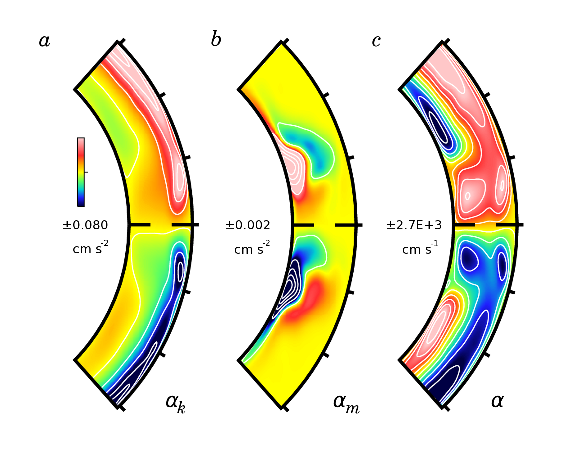
\includegraphics[width=0.7\linewidth]{figs/chapter_7/Figure_15/Figure_15.eps}
  \end{center}
  \vskip-0.25cm
  \caption[Estimating the mean-field $\alpha$-effect in case~D3]
          {Estimating the mean-field $\alpha$-effect in case~D3.  
    $(a)$~Fluctuating kinetic helicity $\alpha_k$. 
    $(b)$~Fluctuating magnetic (current) helicity $\alpha_m$. 
    $(c)$~Mean-field $\alpha$, constructed by combining
    $\alpha_k$~and~$\alpha_m$ with a turbulent correlation time $\tau$.
  \label{fig:mean_field_alpha}}
  \vskip-0.5cm
\end{figure}

We form a mean-field emf (right-hand side of eq.~\ref{eq:mean field emf}) by
multiplying our derived $\alpha$ (Fig.~\ref{fig:mean_field_alpha}$c$) with our 
$\langle B_\phi \rangle$ (Fig.~\ref{fig:D3_bphi_production}$a$), 
and show this in Figure~\ref{fig:emf_comparison}$a$.  The turbulent emf $E_\mathrm{FI}$,
which is the left-hand side of  equation~(\ref{eq:mean field emf}),
can be measured in our simulations and is shown again in Figure~\ref{fig:emf_comparison}$b$. 
Although there is some correspondence in the two patterns, there are
significant differences.  In particular, the mean-field emf has peak
amplitudes in the cores of the wreaths (at $\pm 15^\circ$ latitude)
and is negative there.  In contrast, the actual fluctuating
emf given by $E_\mathrm{FI}$ is positive and has its highest
amplitude at the poleward side of the wreaths.  Thus the mean-field
emf predicts an incorrect balance in the generation
terms and would yield a distinctly different mean poloidal magnetic field. 
To assess whether better agreement may be achieved with a
latitude-averaged emf, we average the mean-field emf and $E_\mathrm{FI}$ 
separately over the northern and southern hemispheres and plot these quantities
in Figure~\ref{fig:emf_comparison}$c$.  Though both have a similar positive sense near the base of
the convection zone, the hemisphere-averaged $E_\mathrm{FI}$ becomes
small above $0.8R_\odot$ whereas the averaged mean-field emf $\alpha
\langle B_\phi \rangle$ is large and negative there.  Thus even the averaged
emfs are not in accord.



\begin{figure}[!t]
  \begin{center}
    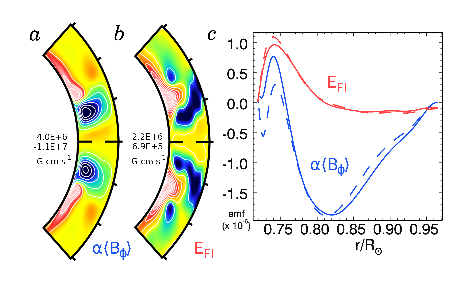
\includegraphics[width=0.9\linewidth]{figs/chapter_7/Figure_16/Figure_16.eps}
  \end{center}
  \caption[Comparison of emfs in case~D3] 
          {Comparison of emfs in case~D3.  
    $(a)$~Profile of proposed mean-field emf given by $\alpha \langle B_\phi \rangle$.
    $(b)$~Actual turbulent emf $E_\mathrm{FI}$ measured in the dynamo.
    $(c)$~Variation of hemisphere-averaged emfs with fractional
    radius.  The mean-field approximated emf is shown in blue, and
    $E_\mathrm{FI}$ in red.  The average over the northern
    hemisphere is shown solid, the southern is dashed.  
  \label{fig:emf_comparison}}
%  \vspace{0.2cm}
\end{figure}

In summary, it is evident that a simple scalar $\alpha$-effect will predict
the wrong sign for the fluctuating emf in the two hemispheres, as 
$\langle B_\phi \rangle$ is anti-symmetric across the equator while
$\langle A_\phi \rangle$ is symmetric.  
An $\alpha$-effect based on the kinetic helicity and magnetic helicity may
capture some sense of the fluctuating emf, as those quantities are
themselves anti-symmetric across the equator.
Yet Figure~\ref{fig:emf_comparison} suggests that there are significant discrepancies
between this particular approximation and our turbulent emf.  In
particular, this mean-field $\alpha$-effect misses
the offset between the generation regions for mean toroidal and mean
poloidal field.  This offset in latitude of the generation regions may
be important for avoiding the $\alpha$-quenching
problems encountered in many mean-field theories.
A more complex mean-field model, which takes spatial gradients
of $\langle B_\phi \rangle$ into account, may do better.  In
particular, the $\vec{\Omega} \cross \vec{J}$-effect
\citep[e.g.,][]{Moffatt&Proctor_1982, Rogachevskii&Kleeorin_2003}
may be at work in these systems, and preliminary explorations indicate
that this term matches the spatial structure of our $E_\mathrm{FI}$
better than the above $\alpha$-effect.  A tensor representation of the
$\alpha$-effect may do much better, and test-field techniques
could be employed to measure this quantity  \citetext{e.g.,
  \citealp{Schrinner_et_al_2005}, and recently reviewed in \citealp{Brandenburg_2009}}.


\section{Production of Fluctuating (Non-Axisymmetric) Field}
Left out of this analysis is the fluctuating component of the
induction equation, which produces the small-scale but strong
fluctuating magnetic fields.  In case~D3 these fields do not appear to
be a dominant feature, but as will be seen in Chapter~\ref{chapter:menagerie of dynamos} 
the fluctuating fields become prominent in our more turbulent dynamo simulations.  
For completeness, we include their induction equation here.
This can be derived by subtracting the mean
induction equation (\ref{eq:mean induction}) from the full induction
equation, yielding the following equation for the fluctuating fields
\begin{eqnarray}\label{eq:ind4}
\frac{\p \vec{B'}}{\p t}&=&~\, ( \langle \BB \rangle \cdot\nab)\vec{v'} + (\vec{B'}\cdot\nab) \langle \VV \rangle  +\, \vec{\EE} \nonumber \\
&~&-( \langle \VV \rangle \cdot\nab)\vec{B'} - (\vec{v'}\cdot\nab) \langle \BB \rangle  -\, \vec{\FF} \nonumber \\
&~&+( \langle v_r \rangle \vec{B'} +  v_r' \langle \BB \rangle)\frac{\p}{\p r}\ln \rb +\, \vec{\GG} \nonumber \\
&~&-\nab\cross(\eta\nab\cross \langle \vec{B'} \rangle ) \thinspace,
\end{eqnarray}
where the quantities $\vec{\EE}=(\vec{B'}\cdot\nab)\vec{v'}- \langle (\vec{B'}\cdot\nab)\vec{v'} \rangle $, 
$\vec{\FF}=(\vec{v'}\cdot\nab)\vec{B'}- \langle (\vec{v'}\cdot\nab)\vec{B'} \rangle $, and 
$\vec{\GG}=(v_r'\vec{B'}- \langle v_r'\vec{B'} \rangle )\frac{\p}{\p r}\ln \rb$, represent the difference between mixed
stresses from which we subtract their axisymmetric mean. In the standard mean-field derivation, these quantities 
are siblings of the G-current involving the mean electromotive force $ \langle \VV\cross\BB \rangle $ and its 3-D equivalent 
$\VV\cross\BB$ \citep[i.e., the so called ``pain in the neck'' term,][]{Moffatt_1978}.


\section{Conclusions}
\label{sec:conclusions}

In our persistent case~D3 we are able to analyze the generation and
transport of mean magnetic field.  We find that our dynamo action is
of an $\alpha-\Omega$ nature, with the mean toroidal fields being
generated by an $\Omega$-effect from the mean shearing flow of
differential rotation.  This generation is balanced by a combination
of turbulent induction and ohmic diffusion.  The mean poloidal fields
are generated by an $\alpha$-effect arising from couplings between the
fluctuating flows and fluctuating fields, with this production largely
balanced by the ohmic diffusion.  This is unlike the toroidal balance,
for here the mean flows play almost no role and the turbulent
correlations are constructive rather than destructive.  In assessing
what a mean-field model might predict for the magnetic structures
realized in case~D3, we find that the isotropic, homogeneous $\alpha$-effect based on kinetic
and magnetic (current) helicities fails to capture the sense of our turbulent
emf.  In general, our $E_\mathrm{FI}$ is poorly represented by an $\alpha
\langle B_\phi \rangle$ that is so determined.



The realization of global-scale magnetic structures in
our simulations, and their great strength relative to the fluctuating
fields, may in part be a consequence of the relatively modest degree
of turbulence attained here.  Whether such structures can be generated
and sustained amidst the far more complex flows in actual stellar
interiors is not yet clear.  If such structures are indeed realized in
stars, they may or may not survive to print
through the highly turbulent convection occurring just below the stellar
photosphere.  If they do appear at the surface, some global-scale
magnetic features may propagate toward the poles along with the bands
of angular velocity speedup.   
There are some indications in stellar observations that
global-scale toroidal magnetic fields may indeed become strong in rapidly
rotating stars \citep{Donati_et_al_2006, Petit_et_al_2008}, though
small-scale fields may still account for much of the magnetic energy
near the surface \citep{Reiners&Basri_2009}.
The global-scale poloidal fields may be more successful in surviving
the passage through the turbulent surface convection.  If they do, the
stellar magnetic field will likely have significant non-dipole components.
Thus the mean poloidal fields observed at the surface may give clues to
the presence of large wreaths of magnetism that occupy the bulk of
the convection zone. 


